% CLAUDE REPORT::WCD-DENSE-0001::2026-11-14T16:40-08:00
% Claude routine "worst-case minimum derivation cost". User follow-up: explore the denser-formula result further.
% Role-neutral and additive. It does NOT edit root main.tex or any TMR/LSPV region.
\documentclass[11pt]{article}
\usepackage{amsmath,amssymb,amsthm,graphicx}
\usepackage[margin=1in]{geometry}
\newtheorem{theorem}{Theorem}
\newtheorem{lemma}[theorem]{Lemma}
\title{WCD-DENSE-0001: a disjointness family for dense 3-SAT and space floors above one assignment}
\author{Claude scheduled routine (worst-case derivation complexity log)}
\date{2026-11-14 16:40 America/Los\_Angeles}
\begin{document}
\maketitle

\paragraph{Status line.}
\begin{itemize}
\item Lemma~\ref{lem:fam} (the family is satisfiable iff $X\cup Z$ misses a triple; fooling set of size $\binom{N}{N/2}$): \textbf{PROVED/EXACT}; exhaustive check for $g=2$ \textbf{COMPUTATIONAL}.
\item Theorem~\ref{thm:ts} ($T\cdot S\ge\Omega(n^{6})$ up to logarithms for sequential-input 3-SAT machines): \textbf{PROVED/EXACT} by the classical crossing-sequence argument. Not independently reviewed. The technique is standard (set disjointness, fooling sets); novelty is not claimed.
\item Correction: the statement in WCD-SPACEFLOOR-0002 that no proved floor rises above $S=n$ is \textbf{FALSIFIED/RETIRED} in general. It holds only for equality-type families.
\item Transfer to random-access input: \textbf{OPEN} (and blocked by the same barrier as before). P versus NP remains \textbf{OPEN}.
\end{itemize}

\section{Why the earlier floor stopped at $n$}
The equality family asks the machine to carry the $k=\Theta(n)$ bits of $a$ across the padding block. Its floor is therefore capped by $n$ at every density: $T\cdot S\ge n\cdot|P|$. But the left part of a formula can hold far more than $n$ bits that matter for satisfiability. A 3-CNF on $n$ variables has up to $8\binom n3$ distinct clauses, and which of them are present can matter individually.

\section{The family}
Let $g\ge2$. Variables $y^{r}_{i}$ for groups $r\in\{0,1,2\}$ and $i<g$.
\begin{itemize}
\item \textbf{Block $C$} (fixed): a ladder encoding forcing exactly one zero in each group, with every clause padded to exactly three literals by fresh variables. It uses $O(g)$ variables and clauses. The assignments of $y$ that survive are the $N=g^{3}$ \emph{triples} $t=(i,j,l)$.
\item The positive clause $D_t=(y^{0}_{i}\vee y^{1}_{j}\vee y^{2}_{l})$ is falsified by exactly the triple $t$.
\item \textbf{Block $P$} (fixed): $N$ distinct positive clauses on $O(g)$ fresh variables.
\item $F_{X,Z}=\{D_t:t\in X\}\;C\;P\;\{D_t:t\in Z\}$ for sets of triples $X,Z$ with $|X|=|Z|=N/2$.
\end{itemize}
Then $n=\Theta(g)$, $L=\Theta(g^{3}\log g)=\Theta(n^{3}\log n)$, and all $F_{X,Z}$ have one length and the same block boundaries.

\begin{lemma}\label{lem:fam}
$F_{X,Z}$ is satisfiable iff $X\cup Z$ is not the set of all triples. The pairs $(X,\overline X)$ are all unsatisfiable, and for $X\ne X'$ at least one of $F_{X,\overline{X'}}$, $F_{X',\overline X}$ is satisfiable.
\end{lemma}
\begin{proof}
A triple $t$ extends to a satisfying assignment iff no present clause is $D_t$, that is iff $t\notin X\cup Z$. For the second claim, $X\cup\overline{X'}$ is everything iff $X'\subseteq X$; with $|X|=|X'|$ and $X\ne X'$ this fails.
\end{proof}

\begin{theorem}\label{thm:ts}
Every machine with a two-way sequential input head that decides 3-SAT in time $T$ and space $S$ satisfies, on this family,
\[T\cdot S\ \ge\ \Omega\bigl(|P|\cdot N\bigr)=\Omega(n^{6}\log n)=\Omega(L^{2}/\log L).\]
With $T=n^{\tau}$, $\tau\ge3$: $S\ge n^{6-\tau}$ up to logarithms. In particular $S>n$ for every $\tau<5$, and linear time in the input length forces $S\approx n^{3}$, which is the input length up to logarithms.
\end{theorem}
\begin{proof}
Fix a cut inside $P$. If $F_{X,\overline X}$ and $F_{X',\overline{X'}}$ had the same crossing sequence there, splicing would make the machine reject both $F_{X,\overline{X'}}$ and $F_{X',\overline X}$, and one of them is satisfiable. So the $\binom N{N/2}=2^{N-O(\log N)}$ sets $X$ have distinct crossing sequences at every cut. A crossing carries $S+O(\log S)$ bits, so at each cut fewer than $2^{N/2}$ sets have a sequence shorter than $N/(3S)$ crossings. A union bound over the $|P|$ cuts leaves a set $X$ with long sequences at every cut, and the time on $F_{X,\overline X}$ is at least $|P|\cdot N/(3S)$.
\end{proof}

\paragraph{General form.} Using only $n^{e}$ of the triples and $n^{d}$ padding clauses ($1\le e,d\le3$) gives $T\cdot S\ge n^{e+d}$ and $S\ge n^{e+d-\tau}$ for $\tau\ge\max(e,d)$. The equality results of WCD-SPACEFLOOR-0002 are the case $e=1$. For $k$-CNF the same construction with $k$ groups gives $T\cdot S\ge n^{2k}$.

\begin{center}
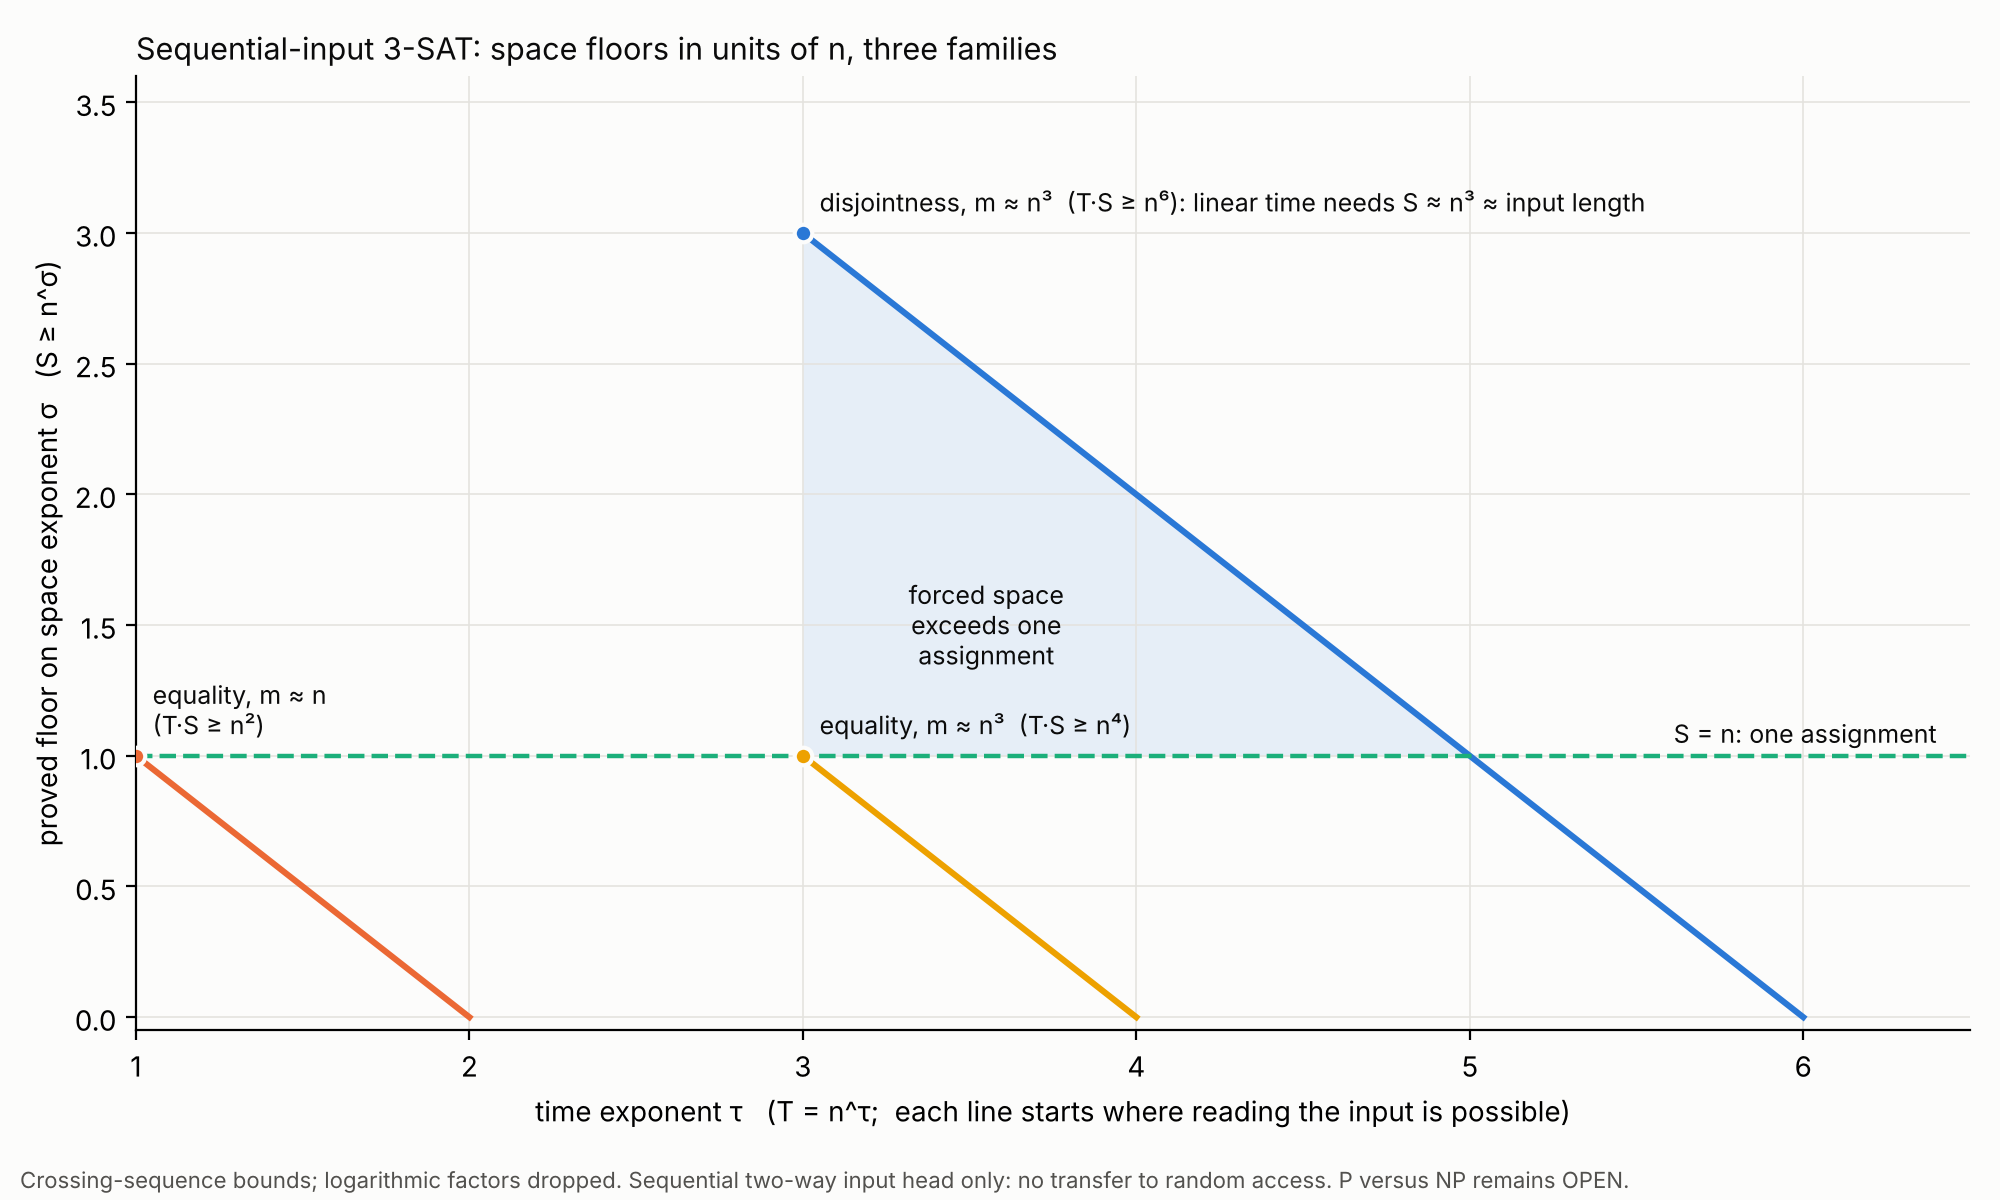
\includegraphics[width=0.9\textwidth]{dense/dense_floors.png}
\end{center}

\section{Reading}
\begin{itemize}
\item \textbf{The cap $S\le n$ was an artefact.} With the disjointness family, a sequential-input algorithm running in time below $n^{5}$ must use more memory than one assignment. Brute force, with exactly $n$ bits, is thereby forced to be slow by a proved bound, though only to time $n^{5}$, not exponential.
\item \textbf{Why:} what must be remembered is not a candidate solution but \emph{which candidates the left half has already excluded}. That is a subset of $n^{3}$ triples, and no summary shorter than about $n^{3}$ bits suffices.
\item \textbf{In input-length units nothing improved.} $T\cdot S\ge L^{2}/\log L$ is the same shape as ONETAPE-0001, and it is the ceiling of the method: one cut carries at most $L$ bits and there are at most $L$ cuts (ONETAPE source note 2).
\item \textbf{No transfer to random access.} A random-access machine re-reads any left clause in one step, so nothing has to be carried across a cut. This is ledger barrier L34.
\item \textbf{Link to the knowledge-width work.} The quantity forced here is the machine's knowledge of the set of excluded candidates, the complement of the alive set of WCD-MCSP-0001. In this model that knowledge cannot be held in few bits, unlike the one-bit wide label of WCD-KWIDTH-0001, because the left half is chosen adversarially from $2^{N}$ sets.
\end{itemize}

\section{CORPUS REVIEWED / DUPLICATION AUDIT / CHANGES}
\begin{itemize}
\item \textbf{Corpus reviewed:} WCD-SPACEFLOOR-0001/0002, WCD-NLIMIT-0001, ONETAPE-0001 with both source notes, WCD-PASS-0001, the consolidated living log.
\item \textbf{Duplication / contradiction audit:} the corpus one-tape work uses equality only; no entry uses disjointness. This report contradicts and corrects the ``no floor above $S=n$'' reading of WCD-SPACEFLOOR-0002 (log item 25) and the matching sentence in WCD-NLIMIT-0001.
\item \textbf{What changed relative to root main:} nothing; \texttt{main.tex} is not edited.
\item \textbf{Adopted:} the crossing-sequence argument of ONETAPE-0001. \textbf{Retired:} the $S\le n$ observation.
\item \textbf{Stale or overstated claims found:} as above.
\end{itemize}

\section{Evidence}
\texttt{dense/disjointness\_family.py}: for $g=2$ ($N=8$), all $70\times70=4900$ pairs checked by DPLL, 0 wrong, one encoded length, 4830 satisfiable, fooling set of size 70 with 0 violations. Sizes for $g=4,\dots,32$: $N/n$ grows from 0.76 to 59; the ratio of the bound to $L^{2}$ settles near 0.007 (logarithm and constants). Output \texttt{dense/raw\_results.json}, figure \texttt{dense/dense\_floors.png}. No TeX engine was available, so this file was not compiled. No literature search was run; set disjointness and fooling sets are textbook.

\paragraph{Next target DN-T1.} Find the largest restricted random-access model in which the excluded-set information still has to be carried: for example a bounded number of input-head reversals per region, or oblivious read schedules. Compare with the multi-pass bound of WCD-PASS-0001.

\medskip\noindent P versus NP remains OPEN. One OPEN load-bearing arrow means P $\ne$ NP is not proved.
\end{document}
% END_OF_VERIFIED_REPORT::CLAUDE::WCD-DENSE-0001
